\chapter{Geometry of smooth and discret space curves}
\section{Introduction}

\note{idée :
Rapprocher l'étude des courbes continues et des discrétisées avec le concept de modèle de la «courbe polygone» de Leibniz et de ses successeurs, une infinité de côtés infiniment petits. \cite[p.235]{Delcourt2011}

Voir aussi que la geometry des space curves semble intimement liée à celle des surface.
\cite{Coolidge2013,Delcourt2011}
}

\blockcquote[Liebniz]{}{Car les courbes n’étant que des polygones d’une infinité de côtés, et ne différent
entre elles que par la différence des angles que ces côtés infiniment petits font
entre eux; il n’appartient qu’à l’Analyse des infiniment petits de déterminer la
position de ces cotés pour avoir la courbure qu’ils forment [...]}.

Attention à la terminologie smooth vs. continious :

\blockquote{A smooth curve is a curve which is a smooth function, where the word "curve" is interpreted in the analytic geometry context. In particular, a smooth curve is a continuous map f from a one-dimensional space to an n-dimensional space which on its domain has continuous derivatives up to a desired order. \footnote{Definition of a smooth curve from mathworld : \url{http://mathworld.wolfram.com/SmoothCurve.html}}
} 

\subsection{Goals and contributions}
Dans ce chapitre, après un bref rappel sur le cadre mathématique d'étude des courbes paramétrique de l'espace, on présente les notions de courbures et de torsion géométrique associées au repère de Frenet. On montre ensuite le cas plus général d'un repère mobile quelconque attaché à une courbe gamma. On définit enfin la particularité d'un repère mobile adapté à un courbe, et on présente, en sus du repère de Frenet, une approche différente pour accrocher des repères le long d'une courbe (Bishop / RMF / Zéro-twisting frame)

Contributions : présentation et comparaison de différentes façons d'estimer la courbure discrete

\subsection{Related work}

\citet{Bishop1975}
\citep{Bishop1975}
\citeauthor{Bishop1975}
\citeyear{Bishop1975}

\cite{Bishop1975}
\cite{Bergou2008}
\cite{Hoffmann2008}
\cite{Bluth2014}
\cite{Frenet1852}
\cite{Delcourt2007}
\cite{Farouki2014}
\cite{Guggenheimer1989}
\cite{Klok1986}

\subsection{Overview}

% --------------------------------------------------------------------------------------------------------------------------------------------
% SMOOTH SPACE CURVE
% --------------------------------------------------------------------------------------------------------------------------------------------


\section{Paramectric curves}

% parametric curve
\subsection{Definition}
Let $I$ be an interval of $\mathbb{R}$ and $F\colon t \mapsto F(t)$ be a map of ${\mathcal{C}}^{}(I,{\mathbb{R}}^3)$. Then $\gamma=(I,F)$ is called a \emph{parametric curve} and :
\begin{itemize}
	\item The 2-uplet $(I,F)$ is called a \emph{parametrization} of $\gamma$
	\item $\gamma = F(I) = \{F(t), t \in I\}$ is called the \emph{graph} or \emph{trace} of $\gamma$
	\item $\gamma$ is said to be ${\mathcal{C}}^{k}$ if $F \in {\mathcal{C}^{k}}^{}(I,{\mathbb{R}}^3)$
\end{itemize}
Note that for a given graph in ${\mathbb{R}}^3$ they may be different possible parameterizations. Thereafter $\gamma$ will simply refers to its graph $F(I)$. 

% regularity
\subsection{Regularity}
Let $\gamma=(I,F)$ be a parametric curve, and $t_0 \in I$ be a parameter.
\begin{itemize}
	\item A point of parameter $t_0$ is called \emph{regular} if $F'(t_0) \neq 0$.
	\\The curve $\gamma$ is called \emph{regular} if $\gamma$ is $\mathcal{C}^{1}$ and $F'(t) \neq 0, \forall t \in I$
	\item A point of parameter $t_0$ is called \emph{biregular} if $F'(t_0)$ and $F''(t_0)$ are not collinear
	\\The curve $\gamma$ is called \emph{biregular} if $\gamma$ is $\mathcal{C}^{2}$ and  $F'(t)\cdot    F''(t) \neq 0, \forall t \in I$
\end{itemize}

% reparametrization
\subsection{Reparametrization}
Let $\gamma=(I,F)$ be a parametric curve of class ${\mathcal{C}}^{k}$, $J \in {\mathbb{R}}^{3}$ an interval, and $\varphi\colon I\mapsto J$ be a ${\mathcal{C}}^{k}$ diffeomorphisme. Lets define $G=F\circ\varphi$. Then :
\begin{itemize}
	\item $G\in{\mathcal{C}}^{k}(J,{\mathbb{R}}^3)$
	\item $G(J)=F(I)$
	\item $\varphi$ is said to be an admissible \emph{change of parameter} for $\gamma$
	\item  $(J,G)$ is said to be another \emph{admissible parametrization} for $\gamma$
\end{itemize}

% natural parametrization
\subsection{Natural parametrization}
Let $\gamma$ be a space curve of class ${\mathcal{C}}^{1}$. A parametrization $(I,F)$ of $\gamma$ is called \emph{natural} if $\|F'(t)\| = 1, \forall t \in I$. Thus :
\begin{itemize}
	\item The curve is necessarily regular
	\item F is strictly monotonic
\end{itemize}

% curve length
\subsection{Curve length}
Let $\gamma=(I,F)$ be a parametric curve of class ${\mathcal{C}}^{1}$. The length of $\gamma$ is define as :
\begin{equation}
	L=\int_{I}\|F'(t)\|dt
\end{equation}
Note that the length of $\gamma$ is invariant under reparametrization.

% arc-length
\subsection{Arc-length parametrization}
Let $\gamma=(I,F)$ be a regular parametric curve. Let $t_0 \in I$ be a given parameter. The following map is said to be the \emph{arc-length of origin $t_0$} of $\gamma$ :
\begin{equation}
	s \colon t \mapsto \int_{t_{0}}^{t}\|F'(u)\|du
	\quad,\quad
	s \in I \times \mathbb{R}
\end{equation}
The arc-length $s \colon I\mapsto s(I)$ is an admissible change of parameter for $\gamma$. Indeed, $s$ is a ${\mathcal{C}}^{1}$ diffeomorphisme because it is bijective ($s'>0$).

Lets define $G=F\circ s^{-1}$ and $J=s(I)$. Thus $(J,G)$ is a natural reparametrization of $\gamma$ and  $\|G'(s)\| = 1, \forall s \in J$. This parametrization is preferred because the natural parameter s traverses the image of $\gamma$ at unit speed\footnote{Regular curves are also known as \emph{unit-speed} curves.} ($\|G'\| = 1$).

Thereafter, for a regular curve $\gamma$ : $\gamma(t)$ will denote the point $F(t)$ of parameter $t \in I$ ; while $\gamma(s)$ will denote the point $G(s)$ of arc-length $s \in J=[0,L]$.

% --------------------------------------------------------------------------------------------------------------------------------------------
% FRENET THRIEDRON
% --------------------------------------------------------------------------------------------------------------------------------------------

\section{Frenet trihedron}\label{sec:frenettrihedron}

%\note{From now, we will assume that the curve $\gamma$ is a regular parametric curve of class ${\mathcal{C}}^{1}$ parametrized by its arc-length $s \in [0,L]$.}

The Frenet trihedron is a fundamental mathematical tool from the field of differential geometry to study local characterization of planar and non-planar space curves. It is a direct orthonormal basis attached to any point $P$, of parameter $t \in I$, on a parametric curve $\gamma$. This basis is composed of three unit vectors $\{\vect{t}(t),\vect{n}(t),\vect{b}(t)\}$ called respectively the \emph{tangent}, the \emph{normal}, and the \emph{binormal} unit vectors\footnote{
Strictly speaking, the map $\fonction{\vect{t}}{t}{\vect{t}(t)}$ is a \emph{vector field} while $\vect{t}(t)$ is a \emph{vector} of $\mathbb{R}^3$. For the sake of simplicity, and if there is no ambiguity, these two notions will not be explicitly distinguished hereinafter.
}.

Introduced by Frenet in 1847 in his thesis \blockcquote[]{Frenet1852}{Courbes à Double Courbure}, it brings out intrinsic local properties of space curves : the curvature ($\kappa$) which evaluates the deviance of $\gamma$ from being a straight line (see \cref{sec:curvature}) ; and the torsion ($\tau_f$) which evaluates the deviance of $\gamma$ from being a planar curve (see \cref{sec:torsion}).

These quantities, also known as \textquote{generalized curvatures} in modern differential geometry, are essential to understand the geometry of space curves. As stated by the \emph{Fundamental Theorem of Space Curves}\footnote{The full demonstration of this theorem is attributed to Darboux in \cite[p.11]{Delcourt2007}.}, a curve is fully determined by its curvature and torsion up to a solid movement in space (see \cref{sec:fundamental}).

% tangent vector
\subsection{Tangent vector}
The first component of the Frenet trihedron is called the \emph{unit tangent vector}. 
Let $\gamma = (I,F)$ be a regular parametric curve. Let $t \in I$ be a parameter. The \emph{unit tangent vector} is defined as :
\begin{equation}
	\vect{t}(t) = \frac{\gamma'(t)}{\|\gamma'(t)\|}
	\quad,\quad
	\|\vect{t}(t)\|=1
\end{equation}
For an arc-length parametrized curve, this expression simply becomes :
\begin{equation}
	\vect{t}(s) = \gamma'(s)
	\quad,\quad
	s \in [0,L]
\end{equation}
In differential geometry, the unit tangente to the curve $\gamma$ at point $P_0$ is obtained as the limit of the (normalized) vector $\overrightarrow{P_0 P}$, as $P$ approches $P_0$ on the path $\gamma$ (\cref{fig:3_1}). For a regular curve, the left-sided and right-sided limits coïncide as $P^-$ and $P^+$ approche $P_0$ respectively from its left and right sides :
\begin{equation}
	\vect{t}(P_0)
	= \lim_{P \to P_0}\frac{\overrightarrow{P_0 P}}{\norm{\overrightarrow{P_0 P}}}
	= \lim_{P^- \to P_0}\frac{\overrightarrow{P_0 P^-}}{\norm{\overrightarrow{P_0 P^-}}}
	= \lim_{P^+ \to P_0}\frac{\overrightarrow{P_0 P^+}}{\|\overrightarrow{P_0 P^+}\|}
\label{eq:3_4}
\end{equation}

\begin{figure}[t]
     \centering
     \subfloat[][Curve's tangent.]{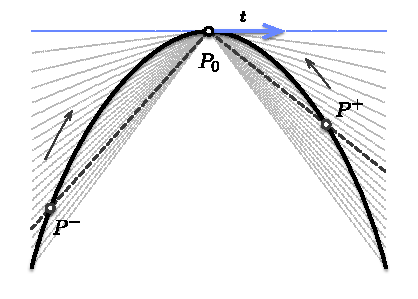
\includegraphics{frenet_tangent.pdf}\label{<figure1>}}
     \subfloat[][Curve's normal and osculating circle.]{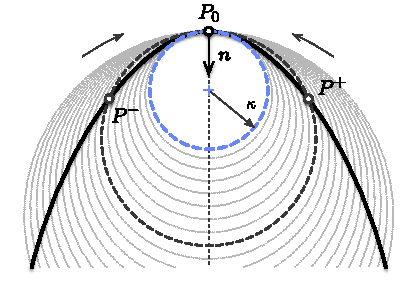
\includegraphics{frenet_normal.pdf}\label{<figure2>}}
     \caption{Differential definition of Frenet's trihedron at given point $P_0$.}
     \label{fig:3_1}
\end{figure}

%Normal vector
\subsection{Normal vector}
The second component of the Frenet trihedron is called the \emph{unit normal vector}. It is constructed from $\vect{t'}$ which is necessarily orthogonal to $\vect{t}$. Indeed :
\begin{equation}
	\|\vect{t}\|=1 \Rightarrow \vect{t^{'}} \cdot  \vect{t} = 0 \Leftrightarrow  \vect{t^{'}} \perp \vect{t}
\end{equation}
Let $\gamma = (I,F)$ be a biregular\footnote{
Note that $\vect{n}$ exists if only $\gamma$ is biregular, that is $\vect{t}'$ never vanishes or, equivalently, $\gamma$ is never locally a straight line.} parametric curve. 
Let $t \in I$ be a parameter. The \emph{unit normal vector} is defined as :
\begin{equation}
	\vect{n}(t) = \frac{\vect{t}'(t)}{\|\vect{t}'(t)\|} 
	= \frac{\gamma'(t) \times (\gamma''(t) \times \gamma'(t))}{\|\gamma'(t)\|^3}
	\quad,\quad
	\|\vect{n}(t)\|=1
\end{equation}
For an arc-length parametrized curve, this expression simply becomes :
\begin{equation}
	\vect{n}(s) = \frac{\vect{t}'(s)}{\|\vect{t}'(s)\|} 
	= \gamma'(s) \times (\gamma''(s) \times \gamma'(s))
	\quad,\quad
	s \in [0,L]
\end{equation}
In differential geometry, the unit normal to the curve $\gamma$ at point $P_0$ is obtained as the limit of the (normalized) vector $\overrightarrow{P_0 P^+}-\overrightarrow{P_0 P^-}$, as $P^-$ and $P^+$ approche $P_0$ respectively from its left and right sides (\cref{fig:3_1}) :
\begin{equation}
	\vect{n}(P_0)
	= \lim_{}\frac{\overrightarrow{P_0 P^+}-\overrightarrow{P_0 P^-}}{\norm{\overrightarrow{P_0 P^+}-\overrightarrow{P_0 P^-}}}
\label{eq:3_4}
\end{equation}
Remark that the notion of \emph{normal vector} is ambiguous for non-planar curves as there is an infinite number of possible normal vectors lying in the plane orthogonal to the curve's tangent. In practice, the tangent derivative is a convenient choice as it allows to extend the notion of curvature from planar to non-planar space curves. However, we will see (\cref{sec:bishop}) that other kind of trihedron can be constructed regarding this choice and that one of them is especially suitable for the study of slender beams.

%Binormal vector and torsion
\subsection{Binormal vector}
The third vector of Frenet's trihedron is called the \emph{unit binormal vector}. It is constructed from $\vect{t}$ and $\vect{n}$ to form an orthonormal direct basis of $\mathbb{R}^{3}$. 
Let $\gamma = (I,F)$ be a biregular parametric curve. Let $t \in I$ be a parameter. The \emph{unit binormal vector} is defined as :
\begin{equation}
	\vect{b}(t) = \vect{t}(t) \times \vect{n}(t)
	= \frac{\gamma'(t) \times \gamma''(t)}{\|\gamma'(t) \times \gamma''(t)\|}
	\quad,\quad
	\|\vect{b}(t)\|=1
\end{equation}
For an arc-length parametrized curve, this expression simply becomes :
\begin{equation}
	\vect{b}(s) = \vect{t}(s) \times \vect{n}(s)
	= \gamma'(s) \times \gamma''(s)
	\quad,\quad
	s \in [0,L]
\end{equation}

% Osculating plane
\subsection{Osculating plane}\label{sec:osculatingplane}
The tangent and normal unit vectors $\{\vect{t},\vect{n}\}$ form an orthonormal basis of the so-called \emph{osculating plane}, whereas the binormal vector $(\vect{b})$ is orthogonal to it. This plane is of prime importance because it is the plane in which the curve takes its curvature (see \cref{sec:curvature}).

As reported in \cite[p.45]{Delcourt2007}, the osculating plane seems to have been first introduced by Bernoulli as the plane passing through three infinitely near points on a curve\footnote{
\blockcquote[p.113]{Bernoulli1728}{Voco autem planum osculans, quod transit per tria curvae quaesitae puncta infinite sibi invicem propinqua}.
}. Likewise, in modern differential geometry, the osculating plane is defined as the limit of the plane passing through the points $P^-$, $P_0$ and $P^+$ while $P^-$ and $P^+$ approche $P_0$ respectively from its left and right side (\cref{fig:3_1}).

Note that the normal unit vector and the binormal unit vector $\{\vect{n},\vect{b}\}$ define the so-called \emph{normal plane}, while the normal tangent vector and the binormal unit vector $\{\vect{t},\vect{b}\}$ define the so-called \emph{rectifying plane}. This planes are secondary for the present study.

% --------------------------------------------------------------------------------------------------------------------------------------------
% CURVE INVARIANTS
% --------------------------------------------------------------------------------------------------------------------------------------------

\section{Curves of double curvature}

The study of space curves belongs to the field of differential geometry. According to \cite[p.28]{Delcourt2007}, the terminology \emph{curve of double curvature} is attributed to Pitot around 1724\footnote{
\blockcquote[p.28]{Pitot1726}{
Les Anciens ont nommé cette courbe Spirale ou Hélice ; parce que la formation sur le cylindre suit la même analogie que la formation d’une spirale ordinaire sur un plan; mais elle est bien différente de la spirale ordinaire, étant une des courbes à double courbure, ou une des lignes qu’on conçoit tracée sur la surface des Solides. Peut-être que ces sortes de courbes à double courbure, ou prises sur la surface des Solides, feront un jour l’objet des recherches des géomètres. Celle que nous venons d’examiner est, je crois, la plus simple de toutes.
}}.
However, as stated in \cite[p.321]{Coolidge2013}, curvature and torsion where probably first thought by Monge around 1771\footnote{
\blockcquote[p.363]{Monge1809}{On appelle point d'inflexion, dans une courbe plane, le point où cette ligne, après avoir été concave dans un sens, cesse de l'être pour devenir concave dans l'autre sens. Il est évident que dans ce point, la courbe perd sa courbure, et que les deux élémens consécutifs sont en ligne droite. Mais une courbe à double courbure peut perdre chacune de ses courbures en particulier, ou les perdre toutes deux dans le même point ; c'est-à-dire, qu'il peut arriver ou que trois élémens consécutifs d'une même courbe à double courbure se trouvent dans un même plan, ou que deux de ces élémens soient en ligne droite. Il suit de là que les courbes à double courbure peuvent avoir deux espèces d'inflexions; la première a lieu lorsque la courbe devient plane, et nous l'appellerons simple inflexion; la seconde, que nous appellerons double inflexion, a lieu lorsque la courbe devient droite dans un de ses points.
}}. It is also interesting to note that, at that time, \textquote{curvature} was also referred to as \textquote{flexure}, reflecting that the study of physical problems (e.g.\ \emph{elastica}) and the study of curves of double curvature were intimately related to each other.

Space curves were historically understood as \emph{curves of double curvature} by extension to the case of planar curves, where the curvature measures the deviance of a curve from being a straight line. The second curvature, nowadays known as the \textquote{torsion} or \textquote{second generalized curvature}, measures the deviance of a curve from being plane. 

%\note{arclength is a Euclidean invariant of the curve.}

\begin{figure}[t]
	\centering
	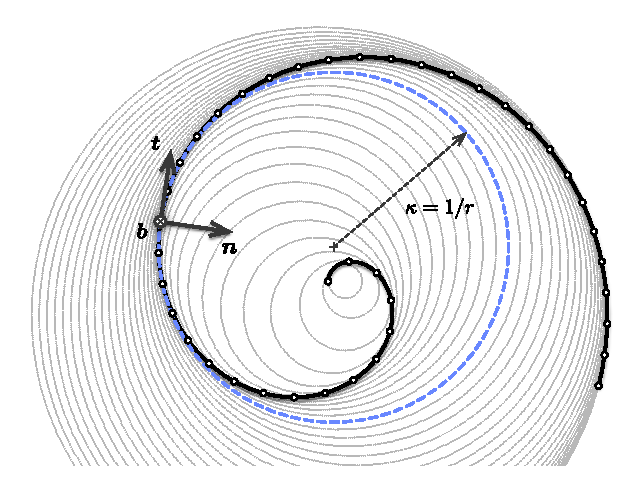
\includegraphics[]{osculating_circle.pdf}
	\caption{Osculating circles for a spiral curve at different parameters.}
	\label{fig:3_2}
\end{figure}

%Curvature
\subsection{First invariant : the curvature}\label{sec:curvature}
In differential geometry, the \emph{osculating circle} is defined as the limit of the circle passing through the points $P^-$, $P_0$ and $P^+$ while $P^-$ and $P^+$ approche $P_0$ (\cref{fig:3_1}). This circle lies on the osculating plane and its radius is nothing but the inverse of the local curvature of a curve\footnote{
As explained by Euler itself, at a given arc-length parameter ($s$), the osculating plane is the plane in which a curve takes its curvature :  
\blockcquote[p.364]{Euler1775}{in quo bina fili elementa proxima in curvantur}.}. While the tangent gives the best local approximation of the curve as a straight line, the osculating circle gives the best local approximation of that curve as an arc.
\subsubsection{Curvature}
Let $\gamma$ be a regular arc-length parametrized curve. Let $s \in [0,L]$ be an arc-length parameter. The \emph{curvature} is a positive scalar quantity defined as :
\begin{equation}
	\kappa(s) = \|\vect{t}'(s)\| \ge 0 
	\quad,\quad
	\vect{t}'(s) = \kappa(s) \vect{n}(s)
\label{eq:curvaturedef}
\end{equation}
The curvature is \emph{independent} regarding the choice of parametrization. This makes the curvature an \emph{intrinsic property} of a given curve and that is why it is also referred to as a \emph{geometric invariant}. Following \cite[pp.203-204]{Gray2006} it can be computed for any parametrization $(I,F)$ of $\gamma$ as :
\begin{equation}
	\kappa(t) = \frac{\|\gamma'(t) \times \gamma''(t) \|}{\|\gamma'(t)\|^3}
	\quad,\quad
	\vect{t}'(t) = \|\gamma'(t)\| \kappa(t) \vect{n}(t)
\label{eq:curvaturedef2}
\end{equation}
Note that in \cref{eq:curvaturedef} the prime denotes the derivative regarding the natural parameter ($s$) while it denotes the derivative regarding any parameter ($t$) in \cref{eq:curvaturedef2}. Consequently, the \emph{speed} of the curve's parametrization appears in the latter equation :
\begin{equation}
	v(t) = \frac{ds}{dt} = \|\gamma'(t)\| = s'(t)
\end{equation}
The curvature measures how much a curve \emph{bends instantaneously} in its osculating plane, that is how fast the tangent vector is rotating in the osculating plane around the binormal vector. In differential geometry this is expressed as :
\begin{equation}
	\kappa(s)
	= \lim_{ds \to 0}\frac{\angle(\vect{t}(s),\vect{t}(s+ds))}{ds}
	= \lim_{ds \to 0}\frac{(\vect{t}(s+ds) - \vect{t}(s)) \cdot \vect{n}(s)}{ds}
\end{equation}
This is equivalent as measuring how fast the osculating plane itself is rotating around the binormal vector. Consequently a curve is locally a \emph{straight line} when its curvature vanishes ($\kappa(s)= 0$).

%Radius of curvature
\subsubsection{Radius of curvature}
The \emph{radius of curvature} is defined as the inverse of the curvature ($r= 1/\kappa$). From a geometric point of view, one can demonstrate that it is the radius of the osculating circle (\cref{fig:3_2}). Remark that where the curvature vanishes the radius of curvature goes to infinity ; that is the osculating circle becomes a line, a circle of infinite radius.

%Osculating circle
\subsubsection{Center of curvature}
The \emph{center of curvature} is defined as the center of the osculating circle (\cref{fig:3_2}). The locus of all the centers of curvature of a curve is called the \emph{evolute}.

\subsubsection{Curvature binormal vector}
Finally, following \cite{Bergou2008} we define the \emph{curvature binormal vector}. Let $\gamma$ be a biregular arc-length parametrized curve. Let $s\in [0,L]$ be an arc-length parameter. The \emph{curvature binormal vector} is defined as :
\begin{equation}
	\vect{\kappa b}(s) = \vect{t}(s) \times \vect{t}'(s) = \kappa(s)\cdot\vect{b}(s)
	\quad,\quad
	\|\vect{\kappa b}(s)\|= \kappa(s)
\end{equation}
This vector will be useful as it embed all the necessary information on the curve's curvature. We will see (\cref{sec:bishopvelocity}) that this vector is associated to the angular velocity of a specific adapted moving frame attached to the curve and called the \emph{Bishop frame}.

% Torsion
\subsection{Second invariant : the torsion}\label{sec:torsion}
Let $\gamma$ be a biregular arc-length parametrized curve. Let $s \in [0,L]$ be an arc-length parameter. The \emph{torsion} is a scalar quantity defined as :
\begin{equation}
	\tau_f(s) = \vect{n}'(s) \cdot \vect{b}(s) = - \vect{b}'(s) \cdot \vect{n}(s)
\end{equation}
The torsion is \emph{independent} regarding the choice of parametrization. This makes the torsion an \emph{intrinsic property} of a given curve and that is why it is also referred to as a \emph{geometric invariant}. Following \cite[p.204]{Gray2006} it can be computed as :
\begin{equation}
	\tau_f(s) = \frac{(\gamma'(s) \times \gamma'(s)) \cdot \gamma''(s)}{\|\gamma'(s) \times \gamma''(s)\|^2}
	\quad when \quad
	\kappa(s) > 0
\end{equation}
The torsion measures how much a curve goes \emph{instantaneously out of its plane}, that is to say how fast the normal or binormal vectors are rotating in the normal plane around the tangent vector. In differential geometry this is expressed as :
\begin{equation}
	\tau_f(s) 
	= \lim_{ds \to 0}\frac{\angle(\vect{n}(s),\vect{n}(s+ds))}{ds}
	= \lim_{ds \to 0}\frac{(\vect{n}(s+ds) - \vect{n}(s)) \cdot \vect{b}(s)}{ds}
\end{equation}
This is equivalent as measuring how fast the osculating plane is rotating around the tangent vector. Consequently a curve is locally \emph{plane} when its torsion vanishes ($\tau_f(s) = 0$).

Remark that the \emph{torsion} is denoted \textquote{$\tau_f$} and not simply \textquote{$\tau$} as the latter will be reserved to denote any angular velocity of a moving adapted frame around its tangent vector. Thus, $\tau_f$ refers to the particular angular velocity of the Frenet trihedron around it's tangent vector. This torsion, which is a geometric property of the curve, will be indifferently referred to as the \emph{torsion of Frenet} or the \emph{geometric torsion}.

% Fundamental theorem of space curves
\subsection{Fundamental theorem of space curves}\label{sec:fundamental}
This two \emph{generalized curvatures}, respectively the curvature ($\kappa$) and the torsion ($\tau_f$), are \emph{invariant} regarding the choice of parametrization and under \emph{euclidean motions}. The \emph{Fundamental theorem of space curves} states that a curve is fully described, up to a Euclidean motion of ${\mathbb{R}}^3$, by its positive curvature ($\kappa > 0$) and torsion ($\tau$) \cite[p.229]{Gray2006}.

% The Serret-Frenet formulas
\subsection{Serret-Frenet formulas}\label{sec:serret}
The \emph{Fundamental theorem of space curves} is somehow a consequence of the \emph{Serret-Frenet formulas}, which is the first-order system of differential equations satisfied by the Frenet trihedron $\{\vect{t},\vect{n},\vect{b}\}$ at any given parameter $s \in J$ :
\begin{equation}
	\left\{
	\begin{aligned}
		&\vect{t^{'}}(s) 	=  \kappa_{}(s) \vect{n}(s)\\
		&\vect{n^{'}}(s) 	=  -\kappa_{}(s) \vect{t}(s) + \tau_f(s) \vect{b}(s) \\
		&\vect{b^{'}}(s) 	=  -\tau_f(s) \vect{n}(s) \\
	\end{aligned}
	\right.
\end{equation}
This system can be seen as the \emph{equations of motion} of the Frenet trihedron moving along the curve $\gamma$. Introducing its \emph{angular velocity vector} also known as the \emph{Darboux vector} ($\vect{\Omega_f}$), the system is expressed as :
\begin{equation}
	\begin{bmatrix}		
		\vect{t^{'}}(s) \\
		\vect{n^{'}}(s) \\
		\vect{b^{'}}(s) \\
	\end{bmatrix}
	=
	\vect{\Omega_f}(s)
	\times
	\begin{bmatrix}		
		\vect{t}(s) \\
		\vect{n}(s) \\
		\vect{b}(s) \\
	\end{bmatrix}
	\quad where \quad
	\vect{\Omega_f}(s)
	=
	\begin{bmatrix}
		\tau(s) \\
		0 \\
		\kappa(s)
	\end{bmatrix}
\end{equation}
Because the Frenet trihedron satisfies a first-order system of differential equations of parameters $\kappa$ and $\tau_f$ it is possible, by integration, to reconstruct the trace of the moving frame and thus the curve, up to a constant of integration (a trihedron in this case). For instance, those classic combinations of curvature and torsion leads to :
\begin{itemize}
	\item a curve of null curvature and null torsion is a straight line ;
	\item a curve of constant curvature and null torsion is a circle ;
	\item a curve of constant curvature and constant torsion is a circular helix.
\end{itemize}

\begin{figure}[t]
	\centering
	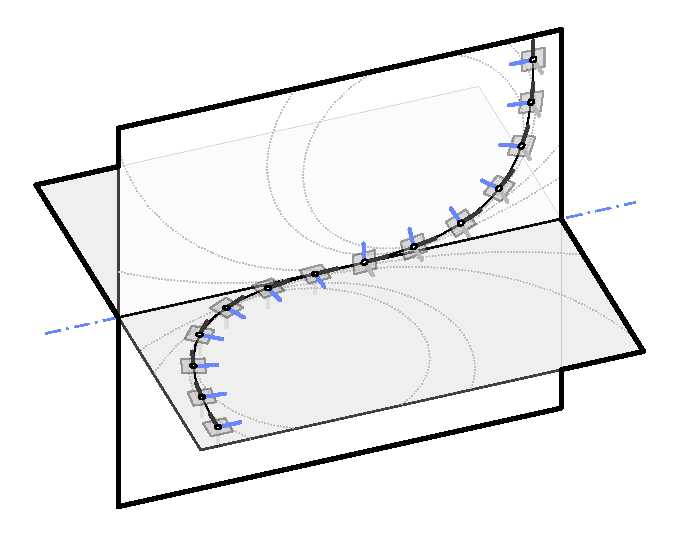
\includegraphics[]{frenet_torsion.pdf}
	\caption{Geometric torsion and rotation of the osculating plane. Note the existence of an inflexion point with a vanishing curvature.}
	\label{fig:3_3}
\end{figure}

% --------------------------------------------------------------------------------------------------------------------------------------------
% CURVE FRAMING
% --------------------------------------------------------------------------------------------------------------------------------------------

\section{Curve framing}

From now, we consider $\gamma=(J,G)$ to be a regular ($\|\gamma'\|=1$) parametric curve of class ${\mathcal{C}}^{2}$, parametrized by its arc-length (denoted $s \in J=[0,L]$). For the sake of simplicity we will refer to $G(s)$ as $\gamma(s)$.

While the Frenet trihedron \blockcquote[p.1]{Bishop1975}{has long been the standard vehicle for analysing properties of the curve invariant\footnote{Namely the curvature ($\kappa$) and the Frenet torsion ($\tau_f$).} under euclidean motions}, a curve can be potentially framed with any arbitrary \emph{moving frame}, understood as an \emph{orthonormal basis field}. Thus, the Frenet frame is not the only way to frame a curve\footnote{Recall the title of Bishop's paper : \blockcquote[]{Bishop1975}{There is more than one way to frame a curve}.} and other frames may or may not exhibit some interesting properties.

In his paper \cite{Bishop1975} Bishop establishes the differential equation that a moving frame must satisfy and remarks that, because of the orthnormality condition, the first derivatives of the frame components can be expressed in terms of themselves through a skew-symmetric coefficient matrix. For such a frame, the understanding of its motion along the curve is thus reduced to the knowledge of only three scalar coefficient functions. He remarks that most of the interesting properties that the Frenet frame exhibits are due to the fact that one of this coefficient function is vanishing everywhere on the curve (that is the frame is \emph{rotation-minimizing} regarding one of its components), and that it is \emph{adapted} to the curve (that is one of its components is nothing but the unit tangent vector).

In this section we introduce the notion of \emph{moving frame} and two properties of interest such a frame can exhibit in addition, that is : to be \emph{adapted} to the curve ; and to be \emph{rotation-minimizing} regrading a given direction. We then reconsider the case of the Frenet frame regrading this mathematical framework. Finally, we introduce the \emph{zero-twisting} frame also known as the \emph{bishop} frame\footnote{Named after Bishop who he introduced it.}. This tool will be fundamental for our study of slender beams.

% moving frame
\subsection{Moving frame}

Let $\gamma : s \rightarrow \gamma(s)$ be an arc-length parametrized curve. A map $F$ which associates to each point of arc-length $s$ a direct orthonormal trihedron is called a \emph{moving frame} :
\begin{equation}
	\fonctionL{F}{[0,L]}{\mathcal{SO}_{3}(\mathbb{R})}{s}{F(s) = \{\vect{e}_{3}(s),\vect{e}_{1}(s),\vect{e}_{2}(s)\}}
\end{equation}
Consequently, a moving frame $F$ attached to $\gamma$ satisfies for all $s \in [0,L]$ :
\begin{equation}
	\left\{
	\begin{aligned}
		& \| \vect{e}_i(s) \| = 1 \\
		& \vect{e}_i(s) \cdot \vect{e}_j(s) = 0\quad , \quad i \neq j
	\end{aligned}
	\right.
\end{equation}
The term \textquote{moving frame} will refer indifferently to the map itself (denoted $F$ or $\{\vect{e}_{3},\vect{e}_{1},\vect{e}_{2}\}$), or to a specific evaluation of the map (denoted $F(s)$ or $\{\vect{e}_{3}(s),\vect{e}_{1}(s),\vect{e}_{2}(s)\}$).

% governing equations
\subsubsection{Governing equations}
Computing the derivatives of the previous relationships leads to the following system of differential equations that the frame must satisfy for all $s \in [0,L]$ :
\begin{equation}
	\left\{
	\begin{aligned}
		&\vect{e}'_i(s) \cdot \vect{e}_i(s) = 0 \\
		&\vect{e}'_{i}(s) \cdot \vect{e}_{j}(s) = -\vect{e}_{i}(s) \cdot \vect{e}'_{j}(s)\quad , \quad i \neq j
	\end{aligned}
	\right.
\end{equation}
Thus, there exists 3 scalar functions ($\tau$, $k_{1}$, $k_{2}$) such that $\{\vect{e}'_{3}, \vect{e}'_{1}, \vect{e}'_{2}\}$ can be expressed in the basis $\{\vect{e}_{3}, \vect{e}_{1}, \vect{e}_{2}\}$ :
\begin{equation}
	\left\{
	\begin{aligned}
		&\vect{e}'_{3}(s) = k_{2}(s)\vect{e}_{1}(s) - k_{1}(s)\vect{e}_{2}(s) \\
		&\vect{e}'_{1}(s) = -k_{2}(s)\vect{e}_{3}(s) + \tau(s)\vect{e}_{2}(s) \\
		&\vect{e}'_{2}(s) = k_{1}(s)\vect{e}_{3}(s) - \tau(s)\vect{e}_{1}(s)
	\end{aligned}
	\right.
\end{equation}
It is common to rewrite this first-order linear system of differential equations\footnote{In the case of a space curve, where $\vect{e}_3$ is chosen to be the curve tangent unit vector and $\vect{e}_1$ is chosen to be the curve normal unit vector, this set of equations is known as the \emph{Serret-Frenet formulas}.}\footnote{In the case of a space curve drawn on a surface, where $\vect{e}_3$ is chosen to be the curve tangent unit vector and $\vect{e}_1$ is chosen to be the surface normal unit vector, this set of equations is known as the \emph{Darboux-Ribaucour formulas}.
} 
as a matrix equation :
\begin{equation}
	\begin{bmatrix}
		\vect{e}'_{3}(s) \\
		\vect{e}'_{1}(s) \\
		\vect{e}'_{2}(s)
	\end{bmatrix}
	=
	\begin{bmatrix}
		0 & k_{2}(s) & -k_{1}(s) \\
		-k_{2}(s) & 0 & \tau(s) \\
		k_{1}(s) & -\tau(s) & 0
	\end{bmatrix}
	\begin{bmatrix}
		\vect{e}_{3}(s) \\
		\vect{e}_{1}(s) \\
		\vect{e}_{2}(s)
	\end{bmatrix}
\label{eq:movingframe}
\end{equation}
Since the progression of any moving frame along $\gamma$ is ruled by a first-order system of differential equations, a unique triplet $\{\tau, k_{1}, k_{2}\}$ leads to a set of moving frames equal to each other within a constant of integration\footnote{
This assumption reminds the \emph{Fundamental theorem of space curves} (\cref{sec:fundamental}).
}. Basically, with a given triplet $\{\tau, k_{1}, k_{2}\}$, one would \guil{propagate} a given initial direct orthonormal trihedron (at $s=0$ for instance) through the whole curve by integrating the system of differential equations. In general, a moving frame will be fully determined by $\tau$, $\kappa_{1}$ and $\kappa_{2}$ together with the initial condition $\{\vect{e}_{3}(s=0),\vect{e}_{1}(s=0),\vect{e}_{2}(s=0)\}$.

% vecteur de Darboux
\begin{figure}[t]
\centering
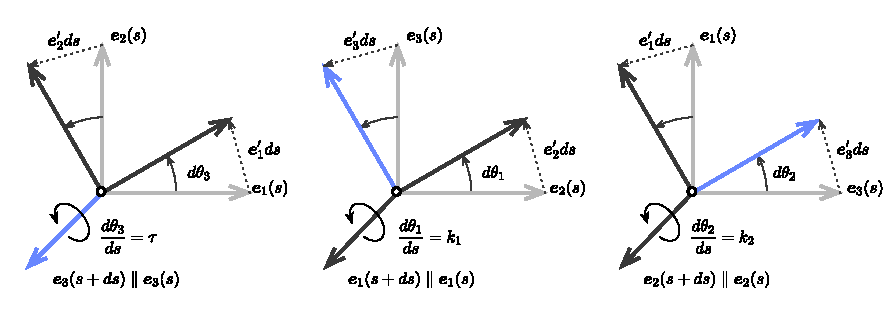
\includegraphics[]{darboux.pdf}
\caption{Geometric interpretation of the Darboux vector of a moving frame.}
\label{fig:3_4}
\end{figure}

\subsubsection{Angular velocity}
It is relevant to consider the mobile frame evolution along $\gamma$ introducing the so-called \emph{Darboux vector} ($\vect{\Omega}$), which corresponds to the instantaneous angular velocity of $F$ at each point of arc-length $s$. Thus, the previous system of differential equations governing the evolution of $F(s)$ along $\gamma$ becomes :
\begin{equation}
	\vect{e}'_{i}(s) = \vect{\Omega}(s) \times \vect{e}_{i}(s)
	\quad avec \quad
	\vect{\Omega}(s)
	=
	\begin{bmatrix}
		\tau(s) \\
		k_1(s) \\
		k_2(s)
	\end{bmatrix}
\end{equation}
This result is straightforward deduced from \cref{eq:movingframe}. Note that the cross product \guil{reveals} that the system is skew-symmetric, which could already be seen in \cref{eq:movingframe}.
Geometrically, decomposing the infinitesimal rotation of the moving frame around its directors between arc-length $s$ and $s+ds$ (\cref{fig:3_4}) shows that the scalar functions $\tau$, $k_{1}$, $k_{2}$ effectively correspond to the angular speed of the frame, respectively around $\vect{e}_{3}$, $\vect{e}_{1}$, $\vect{e}_{2}$ :
\begin{equation}
	\frac{d\theta_3}{ds}(s) = \tau(s)
	\quad,\quad
	\frac{d\theta_1}{ds}(s) = k_{1}(s)
	\quad,\quad
	\frac{d\theta_2}{ds}(s) = k_{2}(s)
\end{equation}

\begin{figure}[t]
\centering
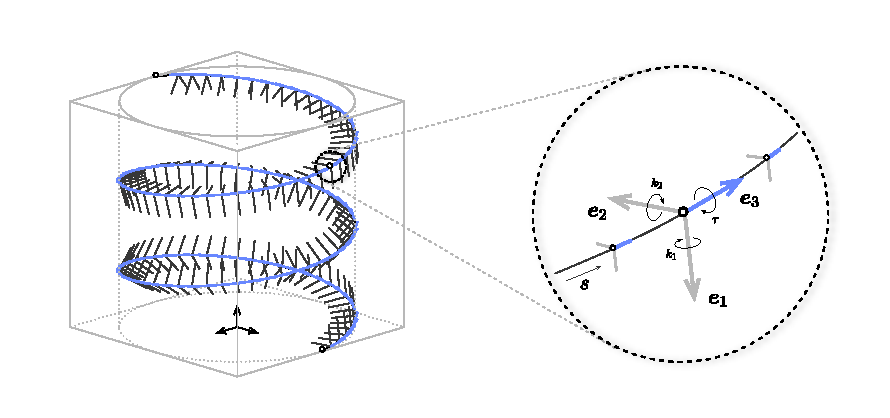
\includegraphics[]{adapted_moving_frame.pdf}
\caption{Adapted moving frame $F(s) =\{\vect{e}_{3}(s),\vect{e}_{1}(s),\vect{e}_{2}(s)\}$ where $\vect{e}_3(s) = \vect{t}(s)$.}
\label{fig:3_5}
\end{figure}

% ADAPTED FRAME
\subsection{Adapted moving frame}
Let $F$ be a moving frame as defined in the previous section. $F$ is said to be \emph{adapted} to $\gamma$ if at each point $\gamma(s)$, $\vect{e}_{3}(s)$ is the unit tangent of $\gamma$ :
\begin{equation}
	\vect{d_{3}}(s) = \vect{t}(s) = \frac{\gamma^{'}(s)}{\|\gamma(s)\|}
	v
\end{equation}
For an adapted frame, the components $k_1$ and $k_2$ of the Darboux vector are related to the curve's curvature. Indeed, recall from \cref{eq:curvaturedef} that $\kappa \equiv \|\gamma''\| = \|\vect{t}'\|$. Or $\vect{t} = \vect{d}_3$ for an adapted frame. Thus, the following relation holds\footnote{\note{Faire le lien avec l'énergie de flexion, qui ne dépend donc que de la géométrie de la courbe dans le cas d'une isotropic rod $\mathcal{E}_b = EI\kappa^2$.}} :
\begin{equation}
	\kappa = \|\vect{d}'_3\| = \sqrt{{k_{1}}^2 + {k_{2}}^2}
\end{equation}

% ROTATION MINIMIZING FRAME
\subsection{Rotation-minimizing frame}
\cite{Wang2008}
Following \cite{Farouki2014} we introduce the notion of \emph{rotation-miniminzing frame}. A frame $\{\vect{e}_{3}$, $\vect{e}_{1}$, $\vect{e}_{2}\}$ is said to be \emph{rotation-miniminzing} regrading a given direction $\vect{d}$ if :
\begin{equation}
	\vect{\Omega}(s) \cdot \vect{d}(s) = 0
	\quad, \quad 
	\forall s \in [0,L]
\end{equation}

% PARALLEL TRANSPORT
\subsection{Parallel transport}
Quid du parallel transport ??
On transporte d'abord le point d'application de $\vect{t1}$ sur $\vect{t2}$. $\vect{t1}$ et $\vect{t2}$ forment un plan de normal $\vect{t1} \times \vect{t2}$. On réaligne $\vect{t1}$ sur $\vect{t2}$ par une rotation d'angle $\angle(\vect{t1},\vect{t2})$ autour de cet axe. La rotation a lieu autour d'un axe perpendiculaire à la fois à $\vect{t1}$ et à $\vect{t2}$. Elle n'implique donc aucune rotation autour des axes $\vect{t1}$ et $\vect{t2}$ eux-mêmes et c'est pourquoi l'on dit que le transport se fait parallèlement de $\vect{t1}$ à $\vect{t2}$.

% FRENET FRAME
\subsection{Frenet frame}

\subsubsection{Definition}
The Frenet frame is a well-known particular adapted moving frame (\cref{sec:frenettrihedron}). At any given regular point $\gamma(s)$ it is defined as the Frenet trihedron $\{\vect{t}(s),\vect{n}(s),\vect{b}(s)\}$ where :
\begin{gather}
\vect{t}(s) = \frac{\gamma^{'}(s)}{\|\gamma'(s)\|}
\quad,\quad
\vect{n}(s) = \frac{\vect{t'}(s)}{\vect{\kappa}(s)}
\quad,\quad
\vect{b}(s)= \vect{t}(s)\times\vect{n}(s)
\end{gather}

\subsubsection{Governing equations}\label{sec:serretfrenet}
The Frenet frame satisfies the \emph{Frenet-Serret} formulas, which govern the evolution of the frame along the curve $\gamma$ :
\begin{equation}
	\begin{bmatrix}
		\vect{t^{'}}(s) \\
		\vect{n^{'}}(s) \\
		\vect{b^{'}}(s)
	\end{bmatrix}
	=
	\begin{bmatrix}
		0 & \kappa_{}(s) & 0 \\
		-\kappa_{}(s) & 0 & \tau_f(s) \\
		0 & -\tau_f(s) & 0
	\end{bmatrix}
	\begin{bmatrix}
		\vect{t}(s) \\
		\vect{n}(s) \\
		\vect{b}(s)
	\end{bmatrix}
\label{eq:3_12}
\end{equation}
One can remember the generic differential equations of an adapted moving frame attached to a curve, where :
\begin{gather}
\vect{d_{3}}(s) = \vect{t}(s) = \frac{\gamma^{'}(s)}{\|\gamma(s)\|}
\quad,\quad
k_{1}(s) = 0
\quad,\quad
k_{2}(s) = \kappa(s)
\quad,\quad
\tau(s) = \tau_{f}(s)
\end{gather}


The Serret-Frenet formulas are a set of three differential equations that the Frenet thriedron satisfies. They can be understood as the motion equations of a moving Frenet trihedron adapted to a space curve $\gamma$. The scalar functions $\kappa$ and $\tau$ are known to be the curvature and the torsion of a the curve $\gamma$ :

\subsubsection{Angular velocity}
Consequently, the angular velocity vector ($\vect{\Omega_{f}}$) of the Frenet frame, also known as the \emph{Darboux vector} in this particular case, is given by :
\begin{equation}
	\vect{\Omega_f}(s)
	=
	\begin{bmatrix}
		\tau_{f}(s) \\
		0 \\
		\kappa(s)
	\end{bmatrix}
\end{equation}
One can remark that the Frenet frame satisfies $\vect{\Omega_f}(s) \cdot \vect{n}(s) = 0$ and is thus a \emph{rotation-miniminzing} frame regarding the normal vector ($\vect{n}$). The motion of this frame through the curve is known as "\emph{pitch-free}".

\subsubsection{Specific points}
The frenet frame has unwanted discontinuities \footnote{\note{montrer un exemple graphique.}} when $\kappa = 0$ and must be ${\mathcal{C}}^{2}$ to be defined \cite{Bloomenthal1990, Wang2008}.

This assertion is equivalent to the well-known \emph{Serret-Frenet formulas}, which give the first-order linear differential equations system that govern the evolution of Frenet's trihedron along a space curve. For a given curvature and torsion, and a given initial trihedron, the geometry of the space curve can be constructed by integration these differential equations.

\footnote{\note{une perturbation de la courbe dans le sens le sens de la courbure engendre une variation de longueur de la courbe proportionnelle à l'inverse de la courbure (au premier ordre) + schéma.}}
\footnote{\note{une perturbation de la courbe dans le sens de la binormale (en tout point) préserve la longueur de la courbe au 1er ordre : c'est un déplacement qui conserve l'hypothèse d'inextensibilité au premier ordre.}}
\footnote{\note{Examiner la question de la fermeture sur une boucle fermée. Schéma.}}

Although it is not possible to define $\vect{n}$ where $\gamma$ is a straight line since $\vect{t}$ is a constant vector and $\vect{t'}$ vanishes ; one can choose to take $\vect{n}$ as a constant vector fields along $\gamma$ and to define the torsion of $\gamma$ to be zero. Although this trihedron does not correspond to the Frenet trihedron (not defined in that case), it will still satisfy the same governing differential equations known as the \emph{Serret-Frenet formulas} (\cref{sec:serretfrenet}).

% BISHOP FRAME
\subsection{Bishop frame}\label{sec:bishop}

\subsubsection{Definition}
Different ways to frame a curve. The usual one is Frenet. But, it could not be as relevant as we want in our field of interest.

The Bishop frame is defined as a a well-known particular adapted moving frame (\cref{sec:frenet}). At any given regular point $\gamma(s)$ it is define as $\{\vect{t}(s),\vect{n}(s),\vect{b}(s)\}$ where :

\cite{Guggenheimer1989}
\cite{Klok1986}
\cite{Bloomenthal1990}
\cite{Wang2008}
\cite{Poston1995}

\blockcquote[p.6]{Wang2008}{The Frenet frame coincides with the RMF for planar
curves, for which $\tau = 0$.}

\blockcquote[p.6]{Wang2008}{Regarder la méthode de la bi-reflexion pour le calcul du repère de bishop}

Although the Frenet frame is not rotation-minimizing with respect to t, one can easily derive such a rotation-minimizing frame from it. New normal-plane vectors (u,v) are specified through a rotation of (p,b) according to u=cos

Bishop frame can be defined relatively to Frenet frame trough a rotation around the unit tangent.
The goal is to nullify the rotation around the tangent. As we know that the Frenet frame is rotating at speed $\tau(s)$ around $\vect{t}(s)$ we just have to rotate back the frenet frame around the tangent vector by the following angle :
\begin{equation}
	\theta(s) = \theta_0(s) - \int_0^s \tau_f(t)dt
\end{equation}
Bishop frame can be expressed relatively to the Frenet frame :
\begin{equation}
	\left\{
	\begin{aligned}
		&\vect{u} = \cos \theta \vect{n} +  \sin \theta \vect{b}\\
		&\vect{v} = -\sin \theta \vect{n} +  \cos \theta \vect{b}
	\end{aligned}
	\right.
\end{equation}
And :
\begin{equation}
	\left\{
	\begin{aligned}
		&\tau =\vect{u^{'}} \cdot \vect{v} = (\vect{\Omega_f} \times \vect{u} + \theta^{'} \vect{v})\cdot  \vect{v} = 0\\
		&k_1 = -\vect{t^{'}} \cdot \vect{v} = -\kappa \vect{n} \cdot \vect{v} = \kappa \sin \theta \\
		&k_2 = \vect{t^{'}} \cdot \vect{u} = \kappa \vect{n} \cdot \vect{u} = \kappa \cos \theta
	\end{aligned}
	\right.
\end{equation}

\subsubsection{Governing equations}
The Bishop frame evolution is governed by the following differential equations :
\begin{equation}
	\begin{bmatrix}
		\vect{t^{'}}(s) \\
		\vect{u^{'}}(s) \\
		\vect{v^{'}}(s)
	\end{bmatrix}
	=
	\begin{bmatrix}
		0 & \kappa(s) \sin \theta(s) & -\kappa(s) \cos \theta(s) \\
		-\kappa(s) \sin \theta(s) & 0 & 0 \\
		\kappa(s) \cos \theta(s) & 0 & 0
	\end{bmatrix}
	\begin{bmatrix}
		\vect{t}(s) \\
		\vect{u}(s) \\
		\vect{v}(s)
	\end{bmatrix}
\label{eq:3_12}
\end{equation}
One can remember the generic differential equations of an adapted moving frame attached to a curve, where :
\begin{gather}
k_{1}(s) = \kappa(s) \sin \theta(s)
\quad,\quad
k_{2}(s) = \kappa(s) \cos \theta(s)
\quad,\quad
\tau(s) = 0
\end{gather}

\subsubsection{Angular velocity}\label{sec:bishopvelocity}
Consequently, the Darboux vector ($\vect{\Omega_{b}}$) of the Bishop frame is given by :
\begin{equation}
	\vect{\Omega_b}(s) = \vect{\kappa b}(s) 
	=
	\begin{bmatrix}
		0\\
		\kappa(s) \sin \theta(s)\\
		\kappa(s) \cos \theta(s)
	\end{bmatrix}
\end{equation}
One can remark that the Bishop frame satisfies $\vect{\Omega_b}(s) \cdot \vect{t}(s) = 0$ and is thus \emph{rotation-miniminzing} regarding the tangent vector. roll-free motion.

\subsubsection{Specific points}
well defined when curvature vanishes

related to mechanical torsion

\note{expliquer la relation entre bishop et frenet : bishop est obtenu par rotation d'un angle $\alpha = \int \tau_f$ par rapport à frenet.

expliquer la notion de parallèle comme l'a formulé Laurent Hauswirth : la projection de $u'$ et $v'$ dans le plan normal à la tangente $t$ est nulle, cad que d'un plan à un autre la projection de $u$ et $v$ est conservée + faire schéma.

Laurent Hauswirth : la complexité d'un problème est en général proportionnelle à la codimension de l'objet étudié et donc, de ce fait les courbes ($codim = 3-1 = 2$) sont des objets plus compliqués que les surfaces ($codim = 3-2=1$) ds $\mathbb{R}^3$.

Expliquer le défaut de fermeture sur une boucle fermée. Calcul du writhe. Quelle différence avec Frenet ?
}

\subsection{Comparison between Frenet and Bishop frames}

\subsubsection{Application A : circular helix}
\begin{equation}
	\left\{
	\begin{aligned}
		\rho = a\\
		z = b\theta
	\end{aligned}
	\right.
\end{equation}

\subsubsection{Application B : conical helix (spiral)}
\begin{equation}
	\left\{
	\begin{aligned}
		\rho = a e^{k\theta}\\
		z = \rho \cot{\alpha}\\
	\end{aligned}
	\right.
\end{equation}


soit pour une spirale dont on connait

\begin{figure}[H]
\centering
\subfloat[][Frenet frame]{%
  \begin{tikzpicture}
\begin{axis}[
	width = 7.5cm,
	xmin=-0.1, xmax= 1.1, restrict x to domain = 0 : 1,
	ymin=-4e-2, ymax= 7e-2, restrict y to domain = -4e-2:6e-2,
	ytick={-3e-2, 0, 3e-2, 6e-2},
	grid=major,
	]

 	\pgfplotstableread{ch3_geometry/plot/frenet_bishop_darboux/frenet.txt}\frenet;
	\addplot [Tblue, smooth, thick]
       	table [x expr=\thisrowno{0}, y expr=\thisrowno{2}] {\frenet};

	\pgfplotstableread{ch3_geometry/plot/frenet_bishop_darboux/frenet.txt}\frenet;
	\addplot [black, smooth, thick, dashed]
       	table [x expr=\thisrowno{0}, y expr=\thisrowno{3}] {\frenet};

	\pgfplotstableread{ch3_geometry/plot/frenet_bishop_darboux/frenet.txt}\frenet;
	\addplot [black, smooth, thick]
       	table [x expr=\thisrowno{0}, y expr=\thisrowno{4}] {\frenet};

\end{axis}
  \end{tikzpicture}}\quad
\subfloat[][Bishop frame]{%
  \begin{tikzpicture}
\begin{axis}[
	width = 7.5cm,
	xmin=-0.1, xmax= 1.1, restrict x to domain = 0 : 1,
	ymin=-4e-2, ymax= 7e-2, restrict y to domain = -4e-2:6e-2,
	ytick={-3e-2, 0, 3e-2, 6e-2},
	grid=major,
	]

       	\pgfplotstableread{ch3_geometry/plot/frenet_bishop_darboux/bishop.txt}\bishop;
	\addplot [Tblue, smooth, thick]
         table [x expr=\thisrowno{0}, y expr=\thisrowno{2}] {\bishop};

         \pgfplotstableread{ch3_geometry/plot/frenet_bishop_darboux/bishop.txt}\bishop;
	\addplot [black, smooth, thick, dashed]
         table [x expr=\thisrowno{0}, y expr=\thisrowno{3}] {\bishop};

         \pgfplotstableread{ch3_geometry/plot/frenet_bishop_darboux/bishop.txt}\bishop;
	\addplot [black, smooth, thick]
         table [x expr=\thisrowno{0}, y expr=\thisrowno{4}] {\bishop};


\end{axis}
  \end{tikzpicture}}
\caption[]{Comparison between Frenet and Bishop frame velocity for a spirale curve.}
\label{fig:3_6}
\end{figure}


\section{Discret curves}

\subsection{Definition and arc-length parametrization}

\subsection{Discret curvature : an equivocal concept}

Curvature is defined from the osculating circle, which is the best approcximation of a curve by a circle.
We can define such a circle and it's radius will be the curvature at that point. Problem : there are several ways to define such a circle.

\subsubsection{Definition}

\note{
Très intéressant de constater que cette vision 3 verticies  vs. 2 edges est déjà présente dès le début dans l'histoire de la compréhension de la courbure.

Pour Euler, le rayon de courbure est le rapport de l’élément d’arc sur l’angle de contin-
gence entre deux tangentes infiniment proches. Par ailleurs, la définition du plan osculateur n’est pas tout à fait lamêmeque chez Bernoulli, plan passant par trois points consécutifs, puis- qu’Euler dit que ce plan contient deux éléments successifs. Il le définit aussi en disant que c’est le plan où la courbe s’incurve. Pour le dire de façon un peu différente : la tangente contient un élément, c’est le lieu où la courbe est droite, la plan osculateur représente l’étape suivante, c’est le lieu où la courbe est arc de cercle. Nous ne pensons pas trahir Euler en faisant cette présen- tation : cela justifie que, pour lui, il est naturel de se placer sur le plan osculateur pour calculer le rayon de courbure. \cite{Delcourt2007}

}

\cite{Hoffmann2008}

The edge osculating circle.
The vertex osculating circle.
La localité est meilleur dans le cas du vertex-based discret osculating circle.
Pour des anlges élevés, le edge-based discret osculating circle est plus pertinent.
La courbure tend vers l'infini quand les 2 edges deviennent colineaires.

La définition du plan osculateur est univoque dans le cas discret : c'est localement le plan défini par 2 edges consécutifs.

Ce n'est pas le cas de la courbure qui perd son côté intrinsèque.

courbure discrete dans le cas général

\subsubsection{Vertex-based osculating circle}

\begin{equation}
	\kappa_1 = \frac{2 \,sin(\varphi_i)}{\|\vect{e}_{i-1} + \vect{e}_{i} \|},
\end{equation}

Problème de convergence lorsque l'angle tend vers pi et que les segments ont même longueur.
En pratique peut probable.

\begin{figure}[]
\begin{center}
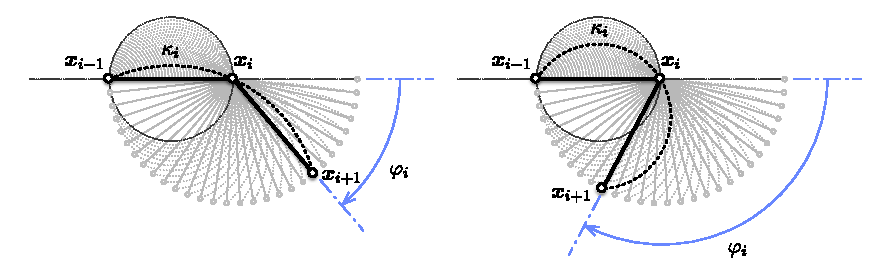
\includegraphics[]{curvature_vertex.pdf}
\caption{Variation of the vertex-based discrete curvature.}
\label{fig:3_7}
\end{center}
\end{figure}

\subsubsection{Edge-based osculating circle}

\begin{equation}
	\kappa_2 = \frac{tan(\varphi_i/2) + tan(\varphi_{i+1}/2)}{\|\vect{e}_{i}\|}
\end{equation}

Bon comportement lorsque l'angle tend vers pi. Demande que les 3 segments soient coplanaires.

\subsubsection{Osculating circle for an arc-length parametrized curve}
\begin{equation}
	\kappa_3 = \frac{2 \,tan(\varphi_i/2)}{l}
	\quad , \quad 
	l = \|\vect{e}_{i} \| = cst
\end{equation}

Qu'on peut réécrire pour des segments de longueur variable, avec la moyenne
\begin{equation}
	\kappa_3 = \frac{2 \,tan(\varphi_i/2)}{l_i}
	\quad , \quad 
	l_i = \frac{\|\vect{e}_{i-1} \| \|\vect{e}_{i} \|}{\|\vect{e}_{i-1}\| + \|\vect{e}_{i}\|}
\end{equation}

\note{
Unlike the smooth case we can not reparameterize a curve. A discrete curve is parameterized by arc-length or it is not \citep[p. 10]{Hoffmann2008}.

Cette condition est extrêmement exigente $\|\vect{e}_{i} \| = cst$. Elle est tenable pour des modèles de poutre non connectées (où le pas de disctrétisation peut-être choisi uniform) mais pour en cas de connexion. Ce point n'est pas éclairci dans les articles de Audoly.
}

\begin{figure}[]
\begin{center}
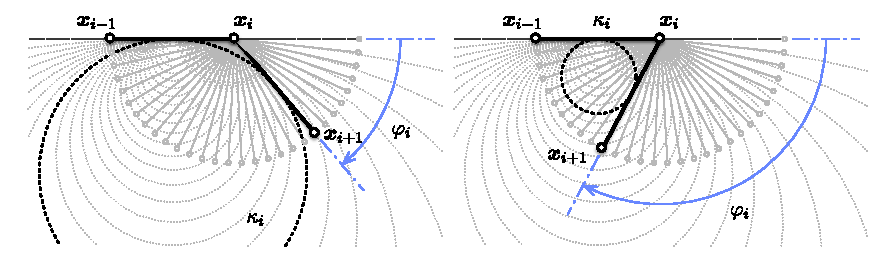
\includegraphics[]{curvature_edge.pdf}
\caption{Variation of the edge-based discrete curvature.}
\label{fig:1_1}
\end{center}
\end{figure}



\begin{figure}[h]
     \centering
     \subfloat[][vertex-based osculating circle]{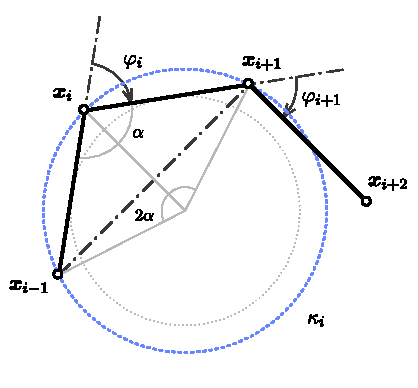
\includegraphics{osculating_circle_vertex.pdf}\label{<figure1>}}
     \subfloat[][edge-based osculating circle]{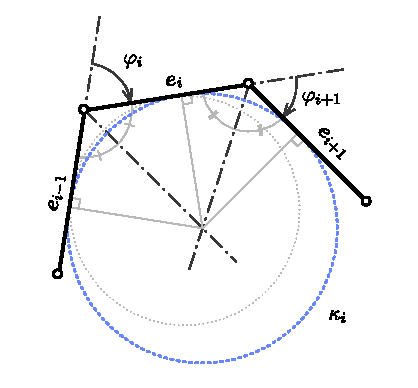
\includegraphics{osculating_circle_edge.pdf}\label{<figure2>}}
     \caption{Definition of the osculating circle for discrete curves.}
     \label{steady_state}
\end{figure}

\begin{figure}[H]
\begin{center}
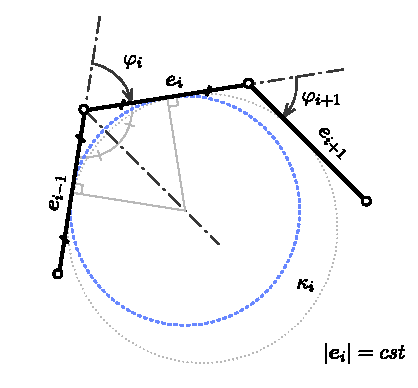
\includegraphics[]{osculating_circle_edge_cst.pdf}
\caption{Another definition of the osculating circle for arc-length parametrized curves.}
\label{fig:1_1}
\end{center}
\end{figure}

\subsection{Variability of discrete curvature regarding $\alpha$}

Qu'on réécrit en posant $\|\vect{e}_{i-1}\| = \alpha \|\vect{e}_{i} \|$, $\alpha \geq 0$ :

\begin{equation}
	\kappa_1 = \frac{2 \,sin(\varphi_i)}{\|\vect{e}_{i}\|(1+ \alpha^2 + 2 \alpha \, cos(\varphi_i))^{1/2}},
	\quad
	\kappa_2 = \frac{4 \,tan(\varphi_i/2)}{\|\vect{e}_{i}\|(1+\alpha)}
\end{equation}

\begin{equation}
	\frac{\kappa_1}{\kappa_2}(\alpha) = \frac{\kappa_1}{\kappa_2}(1/\alpha)= \frac{1+\alpha}{(1+ \alpha^2 + 2 \alpha \, cos(\varphi_i))^{1/2}} \, cos^2(\varphi_i/2)
\end{equation}

\begin{figure}[H]
\begin{center}
\begin{tikzpicture}
\begin{axis}[
	scale only axis,
	legend style={at={(axis cs:0,6)},anchor=north west},
	xmin=-3.1416/4/4, xmax= 3.1416+3.1416/4/4, restrict x to domain = 0 : 3.1416,
	ymin=-2/4, ymax= 10+2/4, restrict y to domain = 0 : 10,
	grid=major,
	axis y line*= left,% the '*' avoids arrow heads
	xlabel={$\varphi$},
	xtick={0, 0.7854, 1.5708, 2.3562, 3.14159},
    	xticklabels={$0$, $\frac{\pi}{4}$,  $\frac{\pi}{2}$,  $\frac{3\pi}{4}$,$\pi$},
	ylabel={$\kappa_1, \kappa_2$},
	ytick={0, 2, 4, 6, 8,10} ]

		% kappa 1
		\addplot[black, samples = 100, domain = 0: 3.1416, solid,  thick]
		{2*sin(deg(x)/2)};
		\node[style={font=\scriptsize}] at (axis cs:3.0,2.4) {$\kappa_1$};
		\addplot[Tgray, samples = 100, domain = 0:3.1416, solid, very thin]					{\curvatureA(deg(x),2)};
		\addplot[color=Tgray, samples = 100, domain = 0:3.1416, solid, very thin]
		{\curvatureA(deg(x),0.5)};

		% kappa 2
		\addplot[black, samples = 400, domain = 0:3.1416, solid,  thick]
		{\curvatureB(deg(x),1)};
		\node[style={font=\scriptsize}] at (axis cs:3.0,9.5) {$\kappa_2$};
		\addplot[color=Tgray, samples = 400, domain = 0:3.1416, solid, very thin]
		{\curvatureB(deg(x),2)};
		\addplot[color=Tgray, samples = 400, domain = 0:3.1416, solid, very thin]
		{\curvatureB(deg(x),0.5)};


	\end{axis}
	\begin{axis}[
	scale only axis,
	xmin=-3.1416/4/4, xmax= 3.1416+3.1416/4/4, restrict x to domain = 0 : 3.1416,
	ymin=-0.2/4, ymax= 1+0.2/4, restrict y to domain = 0 : 1,
	axis y line*=right,
	axis x line=none,
%	ylabel style = {rotate=-90},
	ylabel = {${\kappa_1}/{\kappa_2}$},
	ytick={0, 0.2, 0.4, 0.6, 0.8, 1}
	]
		\addplot[Tblue, samples = 500, domain = 0:3.1416, solid, thick]
		{\curvatureRap(deg(x),1)};
		\node[style={font=\scriptsize}] at (axis cs:1.1,0.95) {$\kappa_1/\kappa_2$};
		\addplot[Tblue, samples = 500, domain = 0:3.1416, solid, very thin]
		{\curvatureRap(deg(x),2)};
	\end{axis}
\end{tikzpicture}

\end{center}
\caption{Discrete curvature comparison for $\alpha \in [0.5,2]$}
\end{figure}

\subsection{Convergence benchmark $\kappa_1$ vs. $\kappa_2$}

\subsubsection{Straight line}

\subsubsection{Circle}

Smooth curve settings:
\begin{equation}
	\mathcal{E} = \int_0^l \kappa^2 ds = \kappa \pi,
	\quad
	l = \pi r,
	\quad
	\kappa = \frac{1}{r}
\end{equation}

Discrete curve :
\begin{equation}
	\varphi_N = \tfrac{\pi}{N},
	\quad
	|\vect{e}| = 2r\sin \tfrac{\varphi}{2},
	\quad
	l_N = N|\vect{e}| =2Nr\sin \tfrac{\varphi}{2} = l \frac{\sin \tfrac{\varphi}{2}}{\tfrac{\varphi}{2}}
\end{equation}

Discrete bending energies :
\begin{equation}
	\mathcal{E}_1 = \mathcal{E} \frac{\sin \tfrac{\varphi}{2}}{\tfrac{\varphi}{2}},
	\quad
	\mathcal{E}_2 = \mathcal{E} \frac{\sin \tfrac{\varphi}{2}}{\tfrac{\varphi}{2} \cos^2 \tfrac{\varphi}{2}},
\end{equation}

Remarque that ratios are independent of scale change (independent of R)

\begin{figure}[H]
\begin{center}
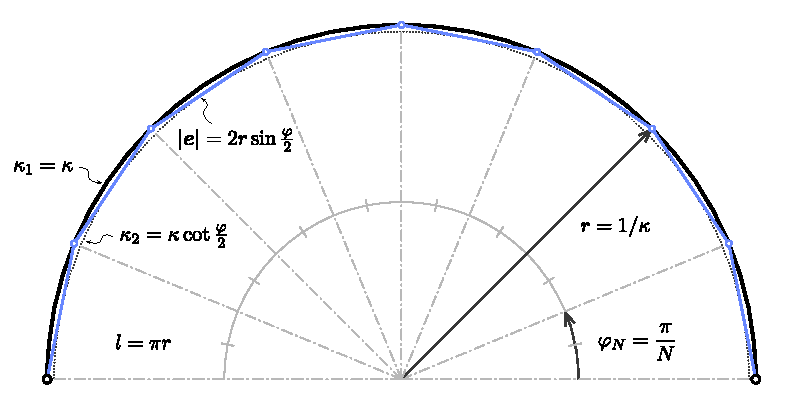
\includegraphics[]{circle.pdf}
\caption{Another definition of the osculating circle for arc-length parametrized curves.}
\label{fig:1_1}
\end{center}
\end{figure}

qsmldkqsmldk s qsd qsd
 sqd
  qs dqs=dlk qs=ldk sq
\newpage
\begin{figure}[]
\begin{center}
\begin{tikzpicture}
	\begin{axis}[
	scale only axis,
	xmin=0, xmax= 21, restrict x to domain = 1 : 20,
	ymin=0.5, ymax= 1.7, restrict y to domain = 0 :1.6,
	grid=major,
	xlabel={$\mathcal{E}_i/\mathcal{E} = f_i(N=l/|e|)$},
	xtick={1,5,10,15,20},
	ylabel={},
	]
		\addplot[black, samples = 1000, domain = 1: 21, solid,  thin]
		{sin(deg(pi/(2*x)))/(pi/(2*x))};
		\node[style={font=\scriptsize}] at (axis cs:3.5,1.565) {$\mathcal{E}_1/\mathcal{E}$};

		\addplot[black, samples = 1000, domain = 1: 21, solid,  thin, dashed]
		{sin(deg(pi/(2*x)))/((pi/(2*x))*cos(deg(pi/(2*x)))^2)};
		\node[style={font=\scriptsize}] at (axis cs:2.5,0.65) {$\mathcal{E}_2/\mathcal{E}$};

		\addplot[Tblue, samples = 1000, domain = 0: 21, solid,  thick]
		{1};
	\end{axis}
\end{tikzpicture}
\end{center}
\caption{Discrete curvature comparison for $\alpha \in [0.5,2]$}
\end{figure}

\subsubsection{Elastica}

\begin{figure}[H]
\begin{center}
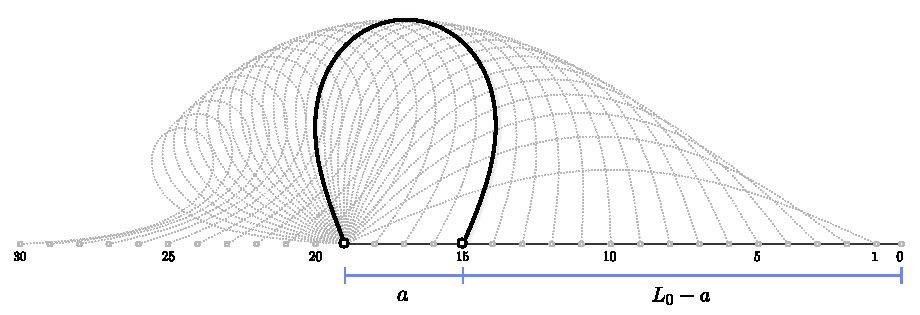
\includegraphics[]{elastica_withnum.pdf}
\caption{Another definition of the osculating circle for arc-length parametrized curves.}
\label{fig:1_1}
\end{center}
\end{figure}

\begin{figure}[H]
\begin{center}
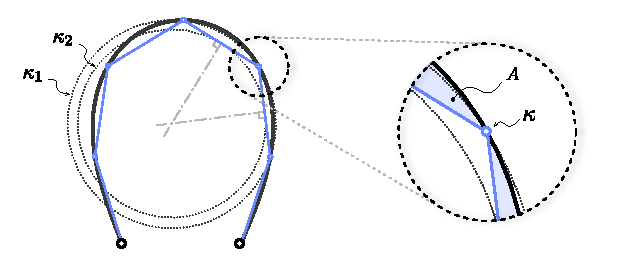
\includegraphics[]{elastica_detail.pdf}
\caption{Another definition of the osculating circle for arc-length parametrized curves.}
\label{fig:1_1}
\end{center}
\end{figure}

\begin{figure}[H]
\centering
\subfloat[][$\mathcal{E}_1/\mathcal{E} = f(N = l/|e|)$]{%
  \begin{tikzpicture}
\begin{axis}[
	width = 7.5cm,
	xmin=8, xmax= 52, restrict x to domain = 10 : 50,
	ymin=0.915, ymax= 1.005, restrict y to domain = 0 :1.6,
	grid=major,
	xtick={0,3,5,10,15,20,25,30,35,40,45,50},
	]

       	\pgfplotstableread{ch3_geometry/plot/discrete_curvature_bench/elastica5.txt}\crvB;
	\addplot [black, smooth, very thin]
       	table [x expr=\thisrowno{0}, y expr=\thisrowno{3}] {\crvB};
%  	\node[Tgray, style={font=\scriptsize}] at (axis cs:9,1) {$5$};

       	\pgfplotstableread{ch3_geometry/plot/discrete_curvature_bench/elastica10.txt}\crvC;
	\addplot [black, smooth, very thin]
        	table [x expr=\thisrowno{0}, y expr=\thisrowno{3}] {\crvC};
    	\node[Tgray, style={font=\scriptsize}] at (axis cs:10,0.985) {$10$};

        \pgfplotstableread{ch3_geometry/plot/discrete_curvature_bench/elastica15.txt}\crvD;
	\addplot [black, smooth, very thin]
         table [x expr=\thisrowno{0}, y expr=\thisrowno{3}] {\crvD};
         \node[Tgray, style={font=\scriptsize}] at (axis cs:10,0.978) {$15$};

     	\pgfplotstableread{ch3_geometry/plot/discrete_curvature_bench/elastica20.txt}	\crvE;
	\addplot [black, smooth, very thin]
       	table [x expr=\thisrowno{0}, y expr=\thisrowno{3}] {\crvE};
       	\node[Tgray, style={font=\scriptsize}] at (axis cs:10,0.965) {$20$};

     	\pgfplotstableread{ch3_geometry/plot/discrete_curvature_bench/elastica25.txt}	\crvF;
	\addplot [black, smooth, very thin]
       	table [x expr=\thisrowno{0}, y expr=\thisrowno{3}] {\crvF};
       	\node[Tgray, style={font=\scriptsize}] at (axis cs:10,0.94) {$25$};

     	\pgfplotstableread{ch3_geometry/plot/discrete_curvature_bench/elastica30.txt}	\crvG;
	\addplot [black, smooth, very thin]
        	table [x expr=\thisrowno{0}, y expr=\thisrowno{3}] {\crvG};
       	\node[Tgray, style={font=\scriptsize}] at (axis cs:15,0.92) {$30$};

         \addplot[Tblue, samples = 100, domain = 0: 50, solid,  thick]
	{1};
\end{axis}
  \end{tikzpicture}}\quad
\subfloat[][$\mathcal{E}_2/\mathcal{E} = f(N = l/|e|)$]{%
  \begin{tikzpicture}
\begin{axis}[
	width = 7.5cm,
	xmin=8, xmax= 52, restrict x to domain = 10 : 50,
	ymin=0.995, ymax= 1.085, restrict y to domain = 1 :1.6,
	grid=major,
	xtick={0,3,5,10,15,20,25,30,35,40,45,50},
	]

         \pgfplotstableread{ch3_geometry/plot/discrete_curvature_bench/elastica5.txt}\crvB;
	\addplot [black, smooth, very thin]
         table [x expr=\thisrowno{0}, y expr=\thisrowno{4}] {\crvB};
         \node[Tgray, style={font=\scriptsize}] at (axis cs:10,1.024) {$5$};

        \pgfplotstableread{ch3_geometry/plot/discrete_curvature_bench/elastica10.txt}\crvC;
	\addplot [black, smooth, very thin]
         table [x expr=\thisrowno{0}, y expr=\thisrowno{4}] {\crvC};
         \node[Tgray, style={font=\scriptsize}] at (axis cs:10,1.044) {$10$};

         \pgfplotstableread{ch3_geometry/plot/discrete_curvature_bench/elastica15.txt}\crvD;
	\addplot [black, smooth, very thin]
         table [x expr=\thisrowno{0}, y expr=\thisrowno{4}] {\crvD};
         \node[Tgray, style={font=\scriptsize}] at (axis cs:10,1.07) {$15$};

     	\pgfplotstableread{ch3_geometry/plot/discrete_curvature_bench/elastica20.txt}	\crvE;
	\addplot [black, smooth, very thin]
         table [x expr=\thisrowno{0}, y expr=\thisrowno{4}] {\crvE};
         \node[Tgray, style={font=\scriptsize}] at (axis cs:13.5,1.08) {$20$};

     	\pgfplotstableread{ch3_geometry/plot/discrete_curvature_bench/elastica25.txt}	\crvF;
	\addplot [black, smooth, very thin]
         table [x expr=\thisrowno{0}, y expr=\thisrowno{4}] {\crvF};
         \node[Tgray, style={font=\scriptsize}] at (axis cs:18,1.08) {$25$};

     	\pgfplotstableread{ch3_geometry/plot/discrete_curvature_bench/elastica30.txt}	\crvG;
	\addplot [black, smooth, very thin]
         table [x expr=\thisrowno{0}, y expr=\thisrowno{4}] {\crvG};
         \node[Tgray, style={font=\scriptsize}] at (axis cs:27,1.08) {$30$};

         \addplot[Tblue, samples = 100, domain = 0: 50, solid,  thick]
	{1};
\end{axis}
  \end{tikzpicture}}
\caption[]{Bending energy representativity}
\label{g:nognot}
\end{figure}

\subsection{Edge versus vertex based tangent vector}

Problème de définition. Facile de définir une tangente sur un edge. Mais une infinité de tangentes possibles à chaque vertex.

So in case of an arc-length parameterized curve the vertex tangent vector points in the same direction as the averaged edge tangent vectors \cite[p. 12]{Hoffmann2008}.

Nous verrons que le cercle 3 points, en plus de mieux représenter l'énergie d'une courbe discrete dans les cas typiques, offre un choix de tangente non ambïgu.


\bibliographystyle{alpha}
\bibliography{../library}
